\documentclass[UTF8]{ctexart}

\usepackage{geometry}
    \geometry{left=4cm,right=4cm,top=2cm,bottom=2cm}
\usepackage{amsmath, amssymb, amsthm}
\usepackage{caption} 	 % 标题
\usepackage{xcolor} 	 % 颜色
\usepackage{graphicx} 	 % 引用图片
\usepackage{float}
\usepackage{multirow}
\usepackage{framed} 	 % 方框 \begin{framed}
\usepackage{indentfirst} 	 % 首行缩进 
    \setlength{\parindent}{0em}
\usepackage{setspace} 	 % 行间距 \begin{spacing}{arg}
\usepackage{extarrows} 	 % 箭头宏包 \xLongrightarrow 
\usepackage{esvect} 	 %向量箭头 \vv{}
\usepackage[version=3]{mhchem} 	 %化学方程式 \ce{}
\usepackage{siunitx} 	 %国际单位 \si{unit} \SI{number}{unit} 

% font
\newcommand{\ve}[1]{\boldsymbol{\mathbf{#1}}}
\newcommand{\unit}[1]{\boldsymbol{\mathbf{\hat{#1}}}}
\newcommand{\mcal}{\mathcal}
\newcommand{\mscr}{\mathscr}
% common symbol
\newcommand{\E}{\mathrm e}
\renewcommand{\I}{\mathrm i}
\newcommand{\R}{\mathbb R}
\newcommand{\Z}{\mathbb Z}
\newcommand{\N}{\mathbb N}
\newcommand{\Q}{\mathbb Q}
\newcommand{\C}{\mathbb C}
% differentiation
\def \DD #1.#2.#3 {\dfrac{d^{#1} #2}{d #3^{#1}}}
\def \PP #1.#2.#3 {\dfrac{\partial^{#1} #2}{\partial #3^{#1}}}
\def \dd #1.#2 {\dfrac{d #1}{d #2}}
\def \pp #1.#2 {\dfrac{\partial #1}{\partial #2}} 
% matrix
\newcommand{\transp}{^{\top}}
\DeclareMathOperator{\tr}{tr}

\pagestyle{empty}

\begin{document}
\section{常数项无穷级数}
\subsubsection{概念}
$ u_1 + u_2 + \cdots + u_n + \cdots $ 的和称为级数, 记作: $ \sum\limits_{n = 1}^{\infty} u_n $ 或 $ \sum u_n $. $ s_n = \sum\limits_{k = 1}^n u_k $ 为该级数的部分和.
\vskip 0.5em
若: $ \lim\limits_{n \to \infty} s_n $ 存在且有限, 极限为 $ s $, 则称级数 $ \sum u_n $ 收敛于 $ s $. 记作 $ \sum\limits_{n = 1}^{\infty} u_n = s < \infty $. 若级数发散于无穷, 则记: $ \sum u_n = \pm\infty $.

\subsubsection{性质}
\begin{framed}
    \begin{itemize}
        \item 若级数 $ \sum u_n = s_u $, $ \sum v_n = s_v$; $ s_u, s_v  \in \overline {\mathbb R} $, 则在不出现未定式($ 0 \cdot \infty, \infty - \infty $)的情况下:
        \[ \sum k u_n = k \sum u_n\]
        \[\sum u_n + \sum v_n = \sum (u_n + v_n) \]
        
        \item 在级数中\textbf{加入, 去掉, 改变有限项}的值, 级数敛散性不改变
        
        \item 级数任意\textbf{加括号}, 保持次序不变, 所得新级数敛散性不改变. 若级数收敛, 则于原级数收敛于同一值
    \end{itemize}
\end{framed}

举例: $ \sum u_n = s $, $ \sum v_n = +\infty $, $ \sum w_n = r $, $ s $ 和 $ r $ 均为有限常数, 则: $ \sum(u_n + v_n) = s + \infty = \infty $, $ \sum(u_n + w_n) = s + r $.

    
\subsection{审敛法}
级数 $ \sum\limits_{n = 1}^{\infty} u_n $ 收敛 $ \Rightarrow $ $ \lim\limits_{n \to \infty} u_n = 0 $. 
\vskip 1em
常用逆否命题判断发散:  $ \lim\limits_{n \to \infty} u_n \neq 0 \Rightarrow $ \textbf{级数发散}

\subsubsection{正项级数}
\begin{framed}
    \begin{itemize}
        \item 正项级数收敛 $ \Leftrightarrow $ 部分和数列有上界
        \item \textbf{比较审敛法}:
        正项级数 $ \sum u_n $ 和 $ \sum v_n $, $ c > 0 $: 
        \[ \text{若 } u_n \leqslant c v_n, \sum v_n \text{ 收敛} \Rightarrow \sum u_n \text{ 收敛}\]
        \[ \text{若 } u_n \geqslant c v_n, \sum v_n \text{ 发散} \Rightarrow \sum u_n \text{ 发散}\]

        \item \textbf{极限比较审敛法}: 
        正项级数 $ \sum u_n $, $ \sum v_n $, $ 0 \leqslant r \leqslant +\infty $:
        \[ \lim_{n \to \infty} \frac{u_n}{v_n} = r 
        \begin{cases}
        \sum v_n \text{ 收敛}, r < +\infty &\Rightarrow \sum u_n \text{ 收敛} \\
        \sum v_n \text{ 发散}, r > 0 &\Rightarrow \sum u_n \text{ 发散}
        \end{cases}\]
    \end{itemize}
\end{framed}

\subsubsection{任意项级数}
\textbf{若} $ \sum |u_n| $ \textbf{收敛}, \textbf{则} $ \sum u_n $ \textbf{必然收敛}, 此时称 $ \sum u_n $ 绝对收敛. 

若 $ \sum |u_n| $ 发散, 而 $ \sum u_n $ 收敛, 则称 $ \sum u_n $ 条件收敛. 

\begin{framed}
    比值审敛法
    \[ \lim\limits_{n\to \infty} \left| \dfrac{u_{n+1}}{u_n} \right| = r \begin{cases}
    {\color{blue} r < 1} & {\color{blue} \text{(绝对)收敛}} \\
    r = 1 & \text{失效} \\
    \text{其他} & \text{发散}
    \end{cases} \]

    根值审敛法
    \[ \lim\limits_{n\to \infty} \sqrt[n]{|u_n|} = r \begin{cases}
    {\color{blue} r < 1} & {\color{blue} \text{(绝对)收敛}} \\
    r = 1 & \text{失效} \\
    \text{其他} & \text{发散}
    \end{cases} \]
\end{framed}




\section{幂级数}
\subsection{收敛半径}
使级数 $\displaystyle \sum f_n (x)  $ 收敛的 $ x $ 取值集合称为该级数的收敛域.
幂级数 $\displaystyle \sum_{n = 0}^{\infty} a_n (x - c)^n $ 的收敛域是以 $ a $ 为中心的一个区间. 即 $ \exists R \in \mathbb R_0^+ $, 有下面三种情况:
\begin{enumerate}
    \item $ |x - c| < R $ 收敛, $ |x - c| > R $ 发散, 端点处不确定. 收敛域举例: $ (c - R, c + R) $
    \item 对任意实数 $ x $ 收敛, 收敛域 $ (-\infty, +\infty) $
    \item 仅 $ x = c $ 收敛, 收敛域 $ \{c\} $
\end{enumerate}
$ R $ 即为收敛半径, 对于后两种情况, 分别记 $ R = \infty $ 和 $ R = 0 $.
\vskip 1em

由比值审敛法(根值审敛法同理), 记 $ \sum a_n x^n $ 系数比 $ a_{n + 1} / a_n $ 的极限 $\displaystyle \lim_{n \to \infty} \left| \dfrac{a_{n + 1}}{a_n} \right| = \rho $, 则收敛半径
\[ R = \frac{1}{\rho} = \begin{cases}
    \dfrac{1}{\rho} &, 0 < \rho < +\infty \\
    \infty &, \rho = 0 \\
    0 &, \rho = + \infty
\end{cases} \]


\subsection{性质}
\subsubsection{加减}
对于幂级数 $\displaystyle \sum_{n = 0}^{\infty} a_n x^n $, $\displaystyle \sum_{n = 0}^{\infty} b_n x^n $, 分别记其收敛半径为 $ R_1 $, $ R_2 $, 则在其公共收敛区间 $ (-R, R), \ R = \min(R_1, R_2)$ 上:
\[ \sum_{n = 0}^{\infty} a_n x^n \pm \sum_{n = 0}^{\infty} b_n x^n = \sum_{n = 0}^{\infty} (a_n \pm b_n) x^n \]

\subsubsection{柯西乘积}
\[ \sum_{n = 0}^{\infty} a_n x^n \cdot \sum_{n = 0}^{\infty} b_n x^n = \sum_{n = 0}^{\infty} c_n x^n \]

其中 $\displaystyle c_n = \sum_{k = 0}^{n} a_k b_{n - k} $.

\subsubsection{求导}
对级数 $\displaystyle f(x) = \sum_{n}^{\infty} a_n x^n $ (收敛半径 $ R $) 有限次求导, 级数的收敛半径不变, 但端点处敛散性可能改变. 即在 $ (-R, R) $ 上:
\[ f'(x) = \sum_{n = 0}^{\infty} (a_n x^n)' = \sum_{n = 0}^{\infty} n a_n x^{n - 1} \]



\subsubsection{积分}
$ (-R, R) $ 上:
\[ \int_0^x f(x) \,dx = \sum_{n = 0}^{\infty}\left( \int_0^x a_n x^n \,dx \right) = \sum_{n}^{\infty} \dfrac{a_n x^{n+1}}{n + 1} \]


\newpage
\section{傅里叶级数}
\subsection{正交函数系}
函数系 $ 1, \cos x, \sin x, \cos 2x, \sin 2x, \dots, \cos nx, \sin nx, \dots $ 中任意两个不同函数之积在 $ [-\pi, \pi] $ 上均为 $ 0 $, 而任意相同函数之积在 $ [-\pi, \pi] $ 上的积分一定非零. 这一特性, 被称为函数系的正交性. 
\[ \int_{- \pi}^\pi 1 \cdot \cos nx \,dx = \int_{- \pi}^\pi 1 \cdot \sin nx \,dx = 0 \]
\[ \int_{- \pi}^\pi \sin mx \cdot \cos nx \,dx = 0 \]
\[ \int_{- \pi}^\pi \sin^2 nx \,dx = \int_{- \pi}^\pi \cos^2 nx \,dx = \pi \]

\subsection{周期为 $ 2 \pi $ 的函数展开}
若 $ f(x) $ 为周期 $ 2 \pi $ 的周期函数, 且满足:
\begin{enumerate}
    \item 一个周期内第一类间断点数量有限
    \item 一个周期类极值点数量有限
\end{enumerate}
换言之, $ f(x) $ 在周期上\textbf{分段连续}, 则对于该函数的任意一点 $ x $:
\[ \dfrac{f(x^-) + f(x^+)}{2} = \dfrac{a_0}{2} + \sum_{n = 1}^{\infty} (a_n \cos nx + b_n \sin nx) \]

其中:
\[ a_n = \dfrac{1}{\pi} \int_{-\pi}^\pi f(x) \cos nx \,dx\]
\[ b_n = \dfrac{1}{\pi} \int_{-\pi}^\pi f(x) \sin nx \,dx\]

记和函数 $\displaystyle s(x) = \dfrac{a_0}{2} + \sum_{n = 1}^{\infty} (a_n \cos nx + b_n \sin nx) $, 则有:
\[ s(x) = \begin{cases}
    \hspace{2.5em} f(x) &, \text{ $ x $ 处连续} \\[0.5em]
    \dfrac{f(x^-) + f(x^+)}{2} &, \text{ $ x $ 处间断}
\end{cases} \]

另外注意:
\[ \begin{array}{ccccccc}
    \text{奇} \times \text{奇} = \text{偶} & & & \text{偶} \times \text{偶} = \text{偶} & & & \text{奇} \times \text{偶} = \text{奇}
\end{array} \]



\newpage
对于仅定义在 $ (-\pi, \pi) $ (或半开半闭, 或闭区间) 上的函数, 可进行周期延拓:
\begin{figure}[H]
    \centering
    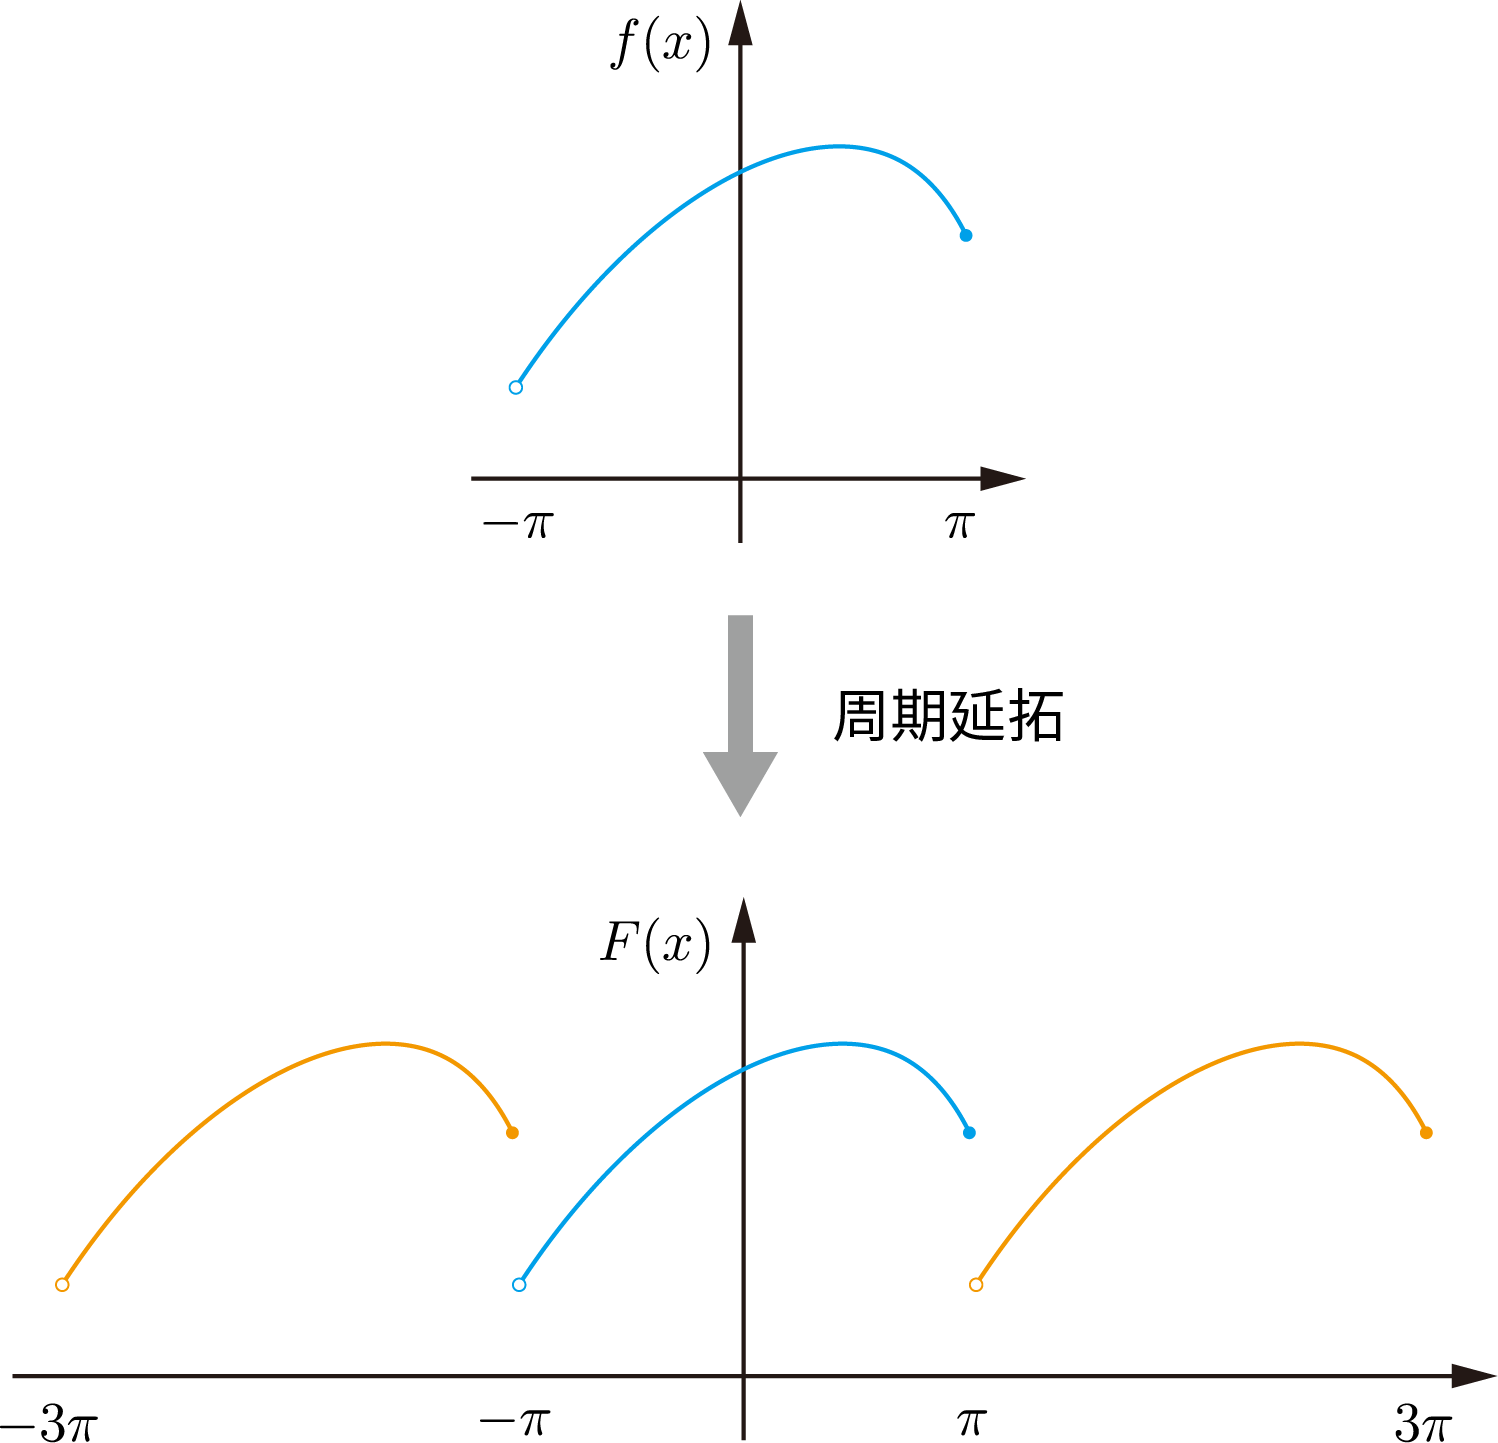
\includegraphics[width = 0.5\linewidth]{periodic_extension}
    \caption*{$ F(x) = f(x), x \in (-\pi, \pi) \qquad F(x) = F(x + 2\pi) , x \in \R $}
\end{figure}

同理对 $ (0, \pi) $ (或半开半闭, 或闭区间) 上的函数也可进行周期延拓. 扩充为 $ (-\pi, \pi) $ 上的奇(偶)函数, 便称为将 $ f(x) $ 作以 $ 2\pi $ 为周期的奇(偶)延拓.

\begin{figure}[H]
    \centering
    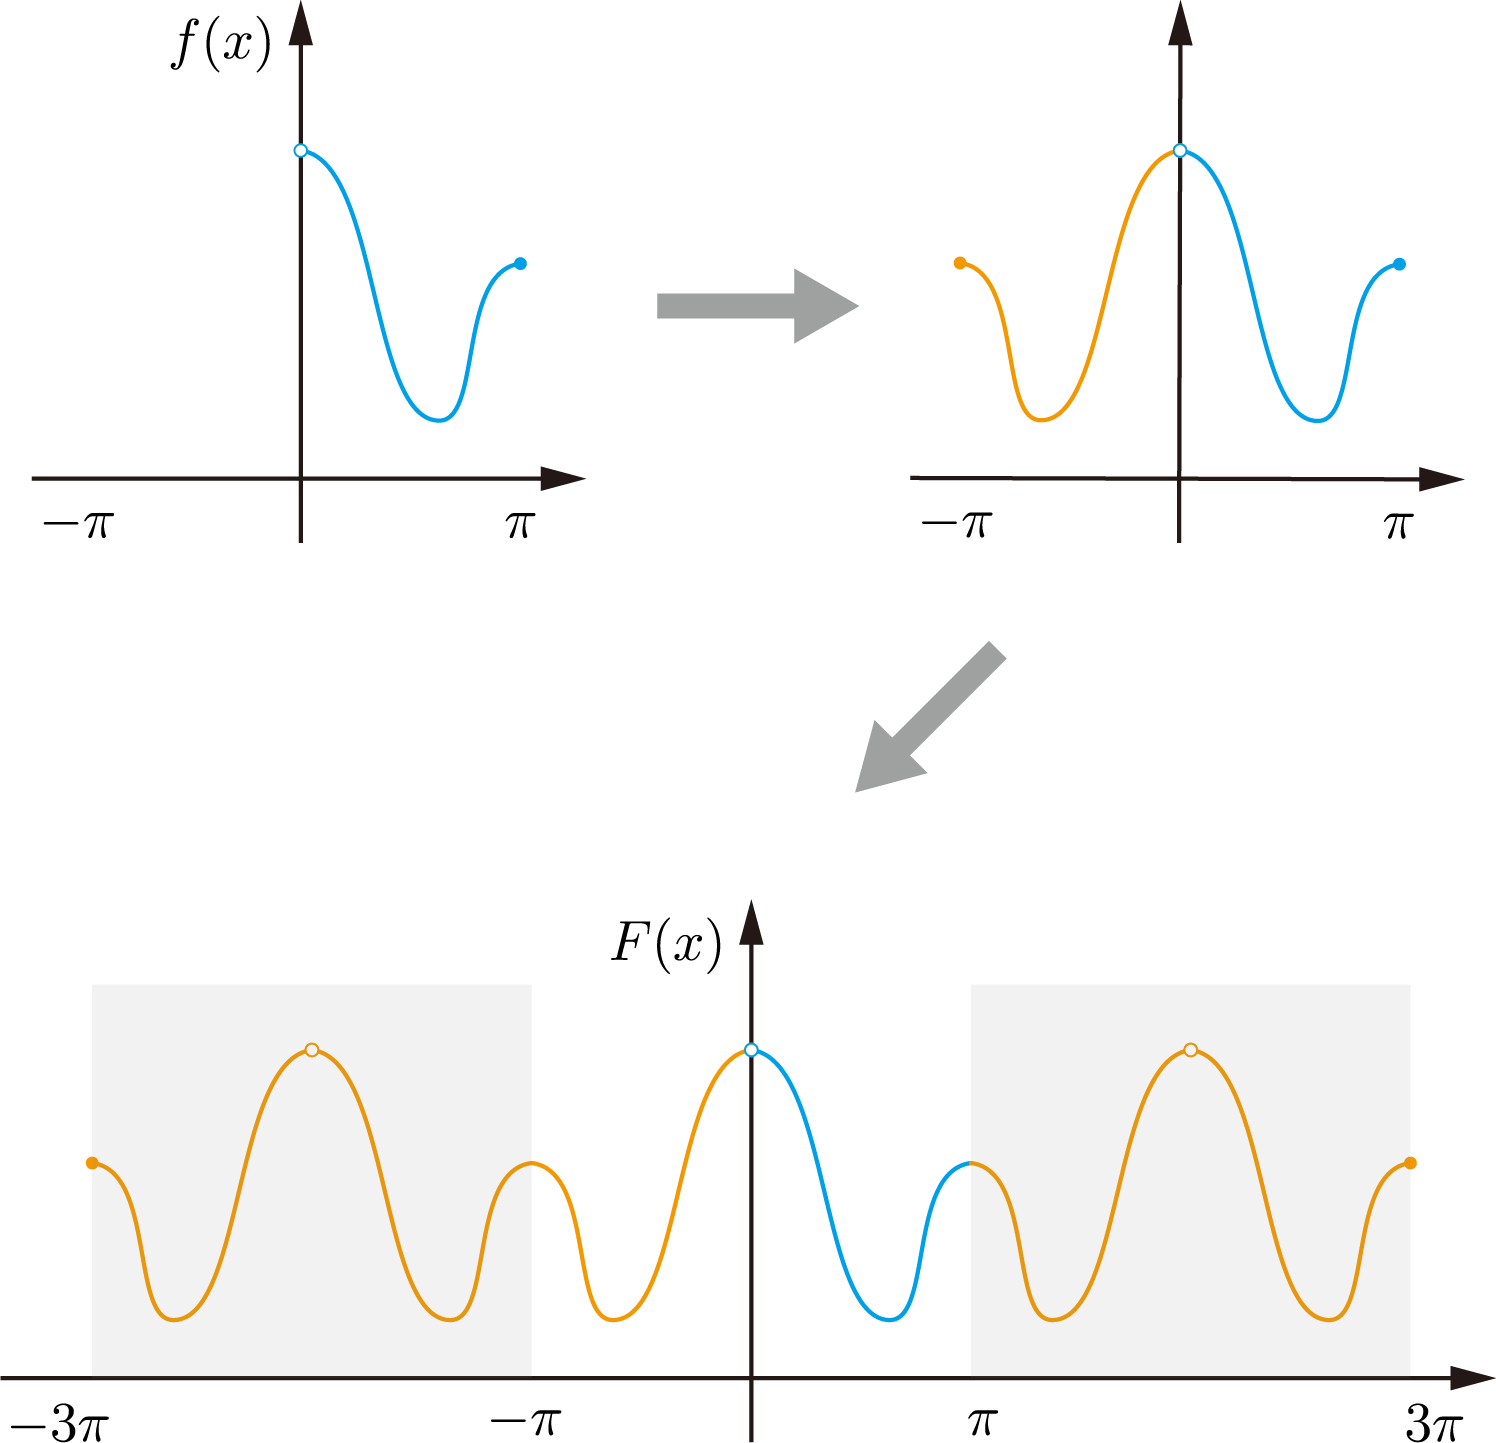
\includegraphics[width = 0.5\linewidth]{periodic_extension2}
    \caption*{一个偶延拓的例子} 
\end{figure}

奇延拓可将傅里叶系数简化:
\[ a_n = \dfrac{1}{\pi} \int_{-\pi}^\pi f(x) \cos nx \,dx = 0 \]
\[ b_n = \dfrac{1}{\pi} \int_{-\pi}^\pi f(x) \sin nx \,dx = \dfrac{2}{\pi} \int_{0}^{\pi} f(x) \sin nx \,dx \]

\newpage
\subsection{周期为 $ 2 L $ 的函数展开}
$ f(x) $ 是周期为 $ 2 L $ 的周期函数, 且满足收敛定理条件, 则级数:
\[ \dfrac{a_0}{2} + \sum_{n = 1}^{\infty}\left( a_n \cos \dfrac{n \pi x}{L} + b_n \sin \dfrac{n \pi x}{L} \right) \]

收敛, 其和函数 $ s(x) $
\[ s(x) = \begin{cases}
    f(x) &, x \text{ 处连续} \\[1em]
    \dfrac{f(x^-) + f(x^+)}{2} &, x \text{ 处间断}
\end{cases}\]

傅里叶系数:
\[ a_n = \dfrac{1}{L} \int_{-L}^L f(x) \cos \dfrac{n \pi x}{L} \,dx \]
\[ b_n = \dfrac{1}{L} \int_{-L}^L f(x) \sin \dfrac{n \pi x}{L} \,dx \]

同理, 奇偶延拓会将傅里叶系数简化.







\newpage
\section{常见幂级数展开及其收敛域}
\begin{framed}
    \begin{enumerate}
        \item $\displaystyle \E^x = \sum_{n = 0}^{\infty} \dfrac{x^n}{n!} $ \hspace{2em} $ (-\infty, +\infty) $
        \item $\displaystyle \sin x = \sum_{n = 0}^{\infty} (-1)^n\dfrac{x^{2n + 1}}{(2n + 1)!} $ \hspace{2em} $ (-\infty, +\infty) $
        \item $\displaystyle \cos x = \sum_{n = 0}^{\infty} (-1)^n \dfrac{x^{2n}}{(2n)!} $ \hspace{2em} $ (-\infty, +\infty) $
        \item $\displaystyle \dfrac{1}{1 - x} = \sum_{n = 0}^{\infty} x^n $ \hspace{2em} $ (-1, 1) $
        \item $\displaystyle \dfrac{1}{1 + x} = \sum_{n = 0}^{\infty} (-1)^n x^n  $ \hspace{2em} $ (-1, 1) $
        \item $\displaystyle \ln(1 - x) = \sum_{n = 0}^{\infty} \dfrac{x^{n+1}}{n + 1}  $ \hspace{2em} $ \big[-1, 1\big) $
        \item $\displaystyle \ln(1 + x) = \sum_{n = 0}^{\infty} \dfrac{(-1)^{n} x^{n+1}}{n + 1}  $ \hspace{2em} $ \big(-1 ,1\big] $
        \item $\displaystyle (1 + x)^\alpha = \sum_{n = 0}^{\infty} \binom{\alpha}{n} x^n = \sum_{n = 0}^{\infty} \dfrac{\alpha^{\underline{n}}}{n!} x^n \qquad ,\binom{\alpha}{n} \text{ 为广义二项式系数} $
        
        其收敛域:\[ \begin{cases}
            (-1, 1) &, \alpha \leqslant -1 \\
            \big( -1, 1 \big] &, -1 < \alpha < 0 \\
            \big[ -1, 1 \big] &, \alpha > 0
        \end{cases} \]
    \end{enumerate}
\end{framed}




\end{document}